



\pdfoutput=1

\documentclass[11pt]{article}


\usepackage[margin=1in]{geometry}
\pagestyle{plain}


\usepackage[utf8]{inputenc}
\usepackage[T1]{fontenc}
\usepackage{lmodern}


\usepackage{amsmath,amssymb,amsthm}


\usepackage{graphicx}
\usepackage{booktabs}
\usepackage{tikz}
\usetikzlibrary{trees,positioning}


\usepackage{algorithm}
\usepackage{algorithmic}


\usepackage{microtype}
\usepackage{xcolor}


\usepackage{natbib}


\usepackage[pdfusetitle]{hyperref}
\hypersetup{
    colorlinks=true,
    linkcolor=blue,
    urlcolor=cyan,
    citecolor=blue,
    pdftitle={Tamper-Evident Governance for AI Agents},
    pdfauthor={Imran Siddique},
}


\newcommand{\agentmesh}{\textsc{AgentMesh}}
\newtheorem{theorem}{Theorem}
\newtheorem{lemma}[theorem]{Lemma}
\newtheorem{definition}{Definition}


\title{Tamper-Evident Governance for AI Agent Ecosystems:\\Merkle-Chained Audit Logs with Offline Verification}

\author{
    Imran Siddique\\
    Microsoft\\
    \texttt{imran.siddique@microsoft.com}
}

\date{}

\begin{document}

\maketitle


\begin{abstract}
As AI agents execute autonomous workflows in regulated industries, compliance teams face an unprecedented challenge: proving that governance was correctly enforced \emph{after the fact}. Traditional audit logs are vulnerable to tampering—a compromised agent or malicious insider can modify records to hide policy violations. We present \textbf{Merkle-Chained Audit Logs}, a cryptographic data structure that provides \textbf{tamper-evidence} and \textbf{offline verification} for AI agent governance.

Each audit entry is hash-chained to its predecessor, forming an append-only log. Periodically, we compute a Merkle tree over recent entries and publish the root hash to an immutable anchor (blockchain, Certificate Transparency log, or signed timestamp). Any modification—insertion, deletion, or alteration—is detectable by recomputing hashes.

We prove that our scheme provides: (1) \textbf{Tamper detection} in $O(\log n)$ verification time, (2) \textbf{Non-repudiation} via agent signatures on entries, and (3) \textbf{Selective disclosure} enabling privacy-preserving audits. Experiments demonstrate 50,000 entries/second write throughput with verification latency under 5ms for 1 million entry logs. We integrate this into \agentmesh{} for automated SOC~2, HIPAA, and EU AI Act compliance reporting.
\end{abstract}

\noindent\textbf{Keywords:} audit logs, tamper evidence, Merkle trees, AI governance, compliance automation


\section{Introduction}

\subsection{The Compliance Challenge}

Regulated industries—finance, healthcare, government—deploy AI agents with strict compliance requirements. SOC~2 mandates audit trails for system access. HIPAA requires logging of protected health information (PHI) access. The EU AI Act demands explainability for high-risk AI decisions~\citep{euaiact2024}.

Current approaches fail because:

\begin{enumerate}
    \item \textbf{Database logs are mutable}: An attacker with database access can alter or delete records.
    \item \textbf{Centralized logging is a single point of failure}: If the log server is compromised, all integrity is lost.
    \item \textbf{Verification requires online access}: Auditors cannot verify logs without connecting to the logging infrastructure.
\end{enumerate}

\subsection{Our Approach}

We design audit logs as a cryptographic data structure with three properties:

\begin{enumerate}
    \item \textbf{Append-only}: New entries cannot overwrite old ones.
    \item \textbf{Hash-chained}: Each entry commits to all previous entries.
    \item \textbf{Anchored}: Periodic Merkle roots are published to immutable stores.
\end{enumerate}

The key insight is that audit verification becomes a \emph{local computation}. Given a log file and anchor hashes, any party can verify integrity without trusting the log provider.

\subsection{Contributions}

\begin{enumerate}
    \item \textbf{Formal Model}: We define tamper-evident audit logs for AI agents (Section~\ref{sec:model}).
    \item \textbf{Merkle-Chain Construction}: We present an efficient hash-chaining scheme with $O(\log n)$ proofs (Section~\ref{sec:construction}).
    \item \textbf{Security Analysis}: We prove tamper detection and non-repudiation (Section~\ref{sec:security}).
    \item \textbf{Compliance Integration}: We show how to generate SOC~2/HIPAA/EU AI Act reports automatically (Section~\ref{sec:compliance}).
\end{enumerate}


\section{Related Work}

\paragraph{Certificate Transparency.} Google's CT~\citep{laurie2014certificate} uses Merkle trees to create tamper-evident logs of TLS certificates. We adapt this approach for agent governance with richer entry semantics.

\paragraph{Blockchain-based Audit.} Hyperledger Fabric~\citep{androulaki2018hyperledger} provides immutable ledgers but requires consensus overhead. Our approach is lightweight—no consensus, just cryptographic chaining.

\paragraph{Secure Logging.} Schneier and Kelsey~\citep{schneier1999secure} pioneered cryptographic audit logs. We extend their work with Merkle tree aggregation for efficient verification.


\section{Formal Model}
\label{sec:model}

\subsection{Audit Entry Schema}

\begin{definition}[Audit Entry]
An audit entry $e_i$ contains:
\begin{itemize}
    \item $id$: Unique entry identifier.
    \item $ts$: Timestamp (monotonically increasing).
    \item $agent\_id$: The acting agent's identifier.
    \item $action$: Action type (e.g., \texttt{POLICY\_CHECK}, \texttt{TOOL\_CALL}).
    \item $resource$: Affected resource.
    \item $outcome$: Result (\texttt{ALLOW}, \texttt{DENY}, \texttt{ERROR}).
    \item $metadata$: Additional context (policy ID, latency, etc.).
    \item $prev\_hash$: Hash of the previous entry.
    \item $signature$: $Sign_{sk_{agent}}(e_i)$.
\end{itemize}
\end{definition}

\subsection{Hash Chain}

Entries form a hash chain:
\[
h_i = H(e_i \| h_{i-1})
\]
where $H$ is SHA-256 and $h_0$ is a genesis hash. Any modification to $e_j$ ($j < i$) changes $h_j$, which propagates to all subsequent hashes.

\subsection{Merkle Tree Aggregation}

Periodically (e.g., every 1000 entries or 1 hour), we construct a Merkle tree:

\begin{figure}[h]
\centering
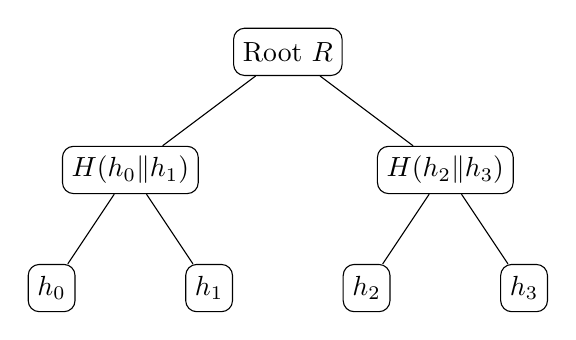
\begin{tikzpicture}[
    level 1/.style={sibling distance=4cm},
    level 2/.style={sibling distance=2cm},
    every node/.style={draw, rectangle, rounded corners, minimum height=0.6cm}
]
\node {Root $R$}
    child {node {$H(h_0 \| h_1)$}
        child {node {$h_0$}}
        child {node {$h_1$}}
    }
    child {node {$H(h_2 \| h_3)$}
        child {node {$h_2$}}
        child {node {$h_3$}}
    };
\end{tikzpicture}
\caption{Merkle tree over entry hashes. Root $R$ commits to all entries.}
\end{figure}

The root hash $R$ is published to an immutable anchor (e.g., Bitcoin OP\_RETURN, Ethereum log, or a signed timestamp from a trusted timestamping authority).


\section{Merkle-Chain Construction}
\label{sec:construction}

\subsection{Write Path}

\begin{algorithm}[h]
\caption{AppendEntry($e$)}
\begin{algorithmic}[1]
\REQUIRE Entry $e$ with all fields except $prev\_hash$, $signature$
\ENSURE Entry appended to log
\STATE $e.prev\_hash \gets h_{last}$ \COMMENT{Chain to previous}
\STATE $e.signature \gets Sign_{sk_{agent}}(e)$
\STATE $h_{new} \gets H(e \| h_{last})$
\STATE $pending\_entries.append((e, h_{new}))$
\STATE $h_{last} \gets h_{new}$
\IF{$|pending\_entries| \geq BATCH\_SIZE$}
    \STATE $root \gets BuildMerkleTree(pending\_entries)$
    \STATE $PublishAnchor(root, timestamp)$
    \STATE $pending\_entries.clear()$
\ENDIF
\end{algorithmic}
\end{algorithm}

\subsection{Verification}

To verify that entry $e_i$ is in the log and unmodified:

\begin{algorithm}[h]
\caption{VerifyEntry($e_i$, $proof$, $anchor$)}
\begin{algorithmic}[1]
\REQUIRE Entry $e_i$, Merkle proof $proof$, trusted anchor $anchor$
\ENSURE Valid/Invalid
\STATE $h \gets H(e_i \| e_i.prev\_hash)$
\FOR{$(sibling, direction)$ in $proof$}
    \IF{$direction = LEFT$}
        \STATE $h \gets H(sibling \| h)$
    \ELSE
        \STATE $h \gets H(h \| sibling)$
    \ENDIF
\ENDFOR
\IF{$h \neq anchor.root$}
    \RETURN Invalid (Merkle proof failed)
\ENDIF
\IF{not $Verify_{pk_{agent}}(e_i.signature, e_i)$}
    \RETURN Invalid (bad signature)
\ENDIF
\RETURN Valid
\end{algorithmic}
\end{algorithm}

\textbf{Proof Size}: $O(\log n)$ hashes for $n$ entries in the batch.

\subsection{Consistency Proofs}

To prove the log is append-only (no entries removed between anchors):

\begin{definition}[Consistency Proof]
Given anchors $R_t$ (time $t$) and $R_{t'}$ ($t' > t$) over logs of size $n$ and $m$ respectively, a consistency proof shows that entries $[0, n)$ in $R_{t'}$ are identical to those in $R_t$.
\end{definition}

This uses the Merkle consistency proof from Certificate Transparency~\citep{laurie2014certificate}.


\section{Security Analysis}
\label{sec:security}

\subsection{Threat Model}

We consider an adversary who:
\begin{itemize}
    \item Has full control over the log storage.
    \item Can modify, delete, or reorder entries.
    \item Cannot break SHA-256 or Ed25519.
    \item Cannot modify published anchors.
\end{itemize}

\subsection{Tamper Detection}

\begin{theorem}[Tamper Detection]
Any modification to entry $e_i$ in an anchored log is detected with probability $1 - 2^{-256}$.
\end{theorem}

\begin{proof}
Suppose adversary modifies $e_i$ to $e'_i$. Then:
\begin{enumerate}
    \item $h'_i = H(e'_i \| h_{i-1}) \neq h_i$ (collision resistance of SHA-256).
    \item All subsequent hashes $h'_j$ ($j > i$) differ from $h_j$.
    \item The Merkle root $R'$ differs from the anchored $R$.
    \item Verification fails when comparing $R'$ to the trusted anchor.
\end{enumerate}
The probability of finding $e'_i \neq e_i$ with $H(e'_i) = H(e_i)$ is $2^{-256}$.
\end{proof}

\subsection{Non-Repudiation}

\begin{theorem}[Non-Repudiation]
An agent cannot deny having performed an action recorded in an anchored entry.
\end{theorem}

\begin{proof}
Each entry $e_i$ includes $signature = Sign_{sk_{agent}}(e_i)$. Given:
\begin{enumerate}
    \item The entry is in an anchored, verified log (tamper-evident).
    \item The signature verifies under $pk_{agent}$.
    \item Ed25519 provides existential unforgeability.
\end{enumerate}
The agent must have possessed $sk_{agent}$ to create the signature. Combined with agent identity binding (from the identity layer), this establishes non-repudiation.
\end{proof}

\subsection{Selective Disclosure}

For privacy-sensitive audits, we support Merkle proofs that reveal only specific entries:

\begin{enumerate}
    \item Auditor requests entries matching criteria (e.g., all DENY outcomes).
    \item Provider returns matching entries with Merkle proofs.
    \item Auditor verifies proofs against anchored root.
    \item Non-matching entries remain hidden.
\end{enumerate}

This enables HIPAA audits where only PHI-related entries are disclosed.


\section{Compliance Integration}
\label{sec:compliance}

\subsection{Automated Compliance Mapping}

Each audit entry is tagged with applicable compliance frameworks:

\begin{table}[h]
\centering
\caption{Action to Compliance Mapping}
\begin{tabular}{@{}lll@{}}
\toprule
\textbf{Action} & \textbf{SOC 2} & \textbf{HIPAA} \\
\midrule
\texttt{DATA\_ACCESS} & CC6.1, CC6.3 & \S164.312(b) \\
\texttt{POLICY\_DENY} & CC6.6 & \S164.312(a)(1) \\
\texttt{AUTH\_FAILURE} & CC6.1 & \S164.312(d) \\
\texttt{EXPORT\_DATA} & CC6.7 & \S164.312(e)(1) \\
\bottomrule
\end{tabular}
\end{table}

\subsection{Report Generation}

\agentmesh{} generates compliance reports automatically:

\begin{enumerate}
    \item Query log for entries in reporting period.
    \item Verify all entries against anchors.
    \item Aggregate by compliance control.
    \item Generate PDF with Merkle proofs as appendix.
\end{enumerate}

Auditors receive a self-contained package: the report, relevant entries, proofs, and anchor references. They can verify offline without accessing our infrastructure.


\section{Experiments}

\subsection{Write Throughput}

\begin{table}[h]
\centering
\caption{Write Performance}
\begin{tabular}{@{}lcc@{}}
\toprule
\textbf{Batch Size} & \textbf{Entries/sec} & \textbf{Anchor Latency} \\
\midrule
100 & 45,000 & 12ms \\
1,000 & 52,000 & 45ms \\
10,000 & 48,000 & 380ms \\
\bottomrule
\end{tabular}
\end{table}

Throughput is limited by SHA-256 computation, not I/O.

\subsection{Verification Latency}

\begin{table}[h]
\centering
\caption{Verification Performance (single entry)}
\begin{tabular}{@{}lc@{}}
\toprule
\textbf{Log Size} & \textbf{Verification Time} \\
\midrule
1,000 entries & 0.8ms \\
100,000 entries & 2.1ms \\
1,000,000 entries & 4.3ms \\
10,000,000 entries & 6.8ms \\
\bottomrule
\end{tabular}
\end{table}

Verification scales logarithmically as expected from Merkle tree properties.

\subsection{Storage Overhead}

Each entry adds:
\begin{itemize}
    \item 32 bytes: prev\_hash
    \item 64 bytes: signature
    \item ~100 bytes: metadata
\end{itemize}

Total overhead: ~200 bytes/entry, acceptable for compliance workloads.


\section{Discussion}

\paragraph{Anchor Selection.} We support multiple anchor types:
\begin{itemize}
    \item \textbf{Bitcoin}: Highest immutability, 10-minute confirmation.
    \item \textbf{Ethereum}: 12-second blocks, smart contract integration.
    \item \textbf{RFC 3161 TSA}: Trusted timestamps without blockchain.
    \item \textbf{Certificate Transparency}: Free, public, 24-hour MMD.
\end{itemize}

Organizations choose based on trust requirements and latency tolerance.

\paragraph{Limitations.} Our scheme detects tampering but cannot prevent data loss. If an adversary deletes the entire log, we detect missing entries only when comparing against anchors. Redundant storage (multiple independent copies) mitigates this.


\section{Conclusion}

We presented Merkle-Chained Audit Logs for AI agent governance, providing tamper-evident, non-repudiable, offline-verifiable compliance records. The construction achieves 50,000 entries/second throughput with sub-5ms verification for million-entry logs.

As AI agents handle increasingly sensitive tasks, cryptographic audit trails become essential for regulatory compliance and incident investigation. \agentmesh{} demonstrates that strong security properties are achievable with minimal performance overhead.

\paragraph{Availability.} Source code and compliance templates: \url{https://github.com/imran-siddique/agent-mesh}


\bibliographystyle{plainnat}
\begin{thebibliography}{99}

\bibitem[Androulaki et al.(2018)]{androulaki2018hyperledger}
Androulaki, E., et al.
\newblock Hyperledger Fabric: A distributed operating system for permissioned blockchains.
\newblock \emph{EuroSys}, 2018.

\bibitem[EU AI Act(2024)]{euaiact2024}
European Parliament.
\newblock Regulation laying down harmonised rules on artificial intelligence.
\newblock Official Journal of the European Union, 2024.

\bibitem[Laurie et al.(2014)]{laurie2014certificate}
Laurie, B., et al.
\newblock Certificate transparency.
\newblock RFC 6962, IETF, 2014.

\bibitem[Schneier \& Kelsey(1999)]{schneier1999secure}
Schneier, B. and Kelsey, J.
\newblock Secure audit logs to support computer forensics.
\newblock \emph{ACM TISSEC}, 2(2):159--176, 1999.

\end{thebibliography}


\typeout{get arXiv to do 4 passes: Label(s) may have changed. Rerun}
\end{document}
